\documentclass[tikz,border=5mm,12pt]{standalone}
\usepackage[fontsize=16pt]{fontsize}
\usetikzlibrary{arrows.meta}

\def\ysep{6mm}
\def\xsep{18mm}
\def\textYsep{24pt}

\begin{document}
  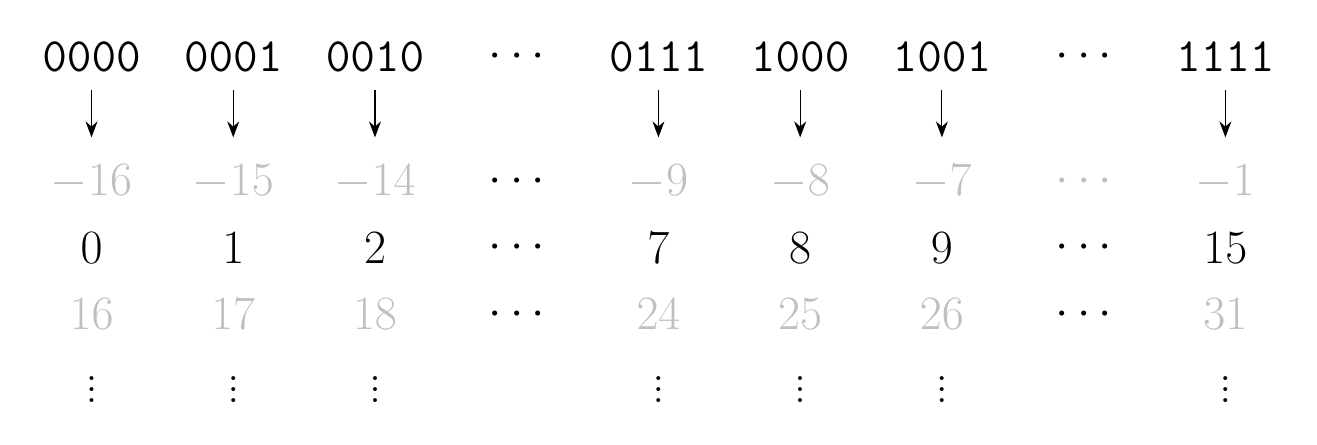
\begin{tikzpicture}[
    arrowtip/.style={
      -{Stealth[scale=1.2]}
    }
  ]
    \node at (0*\xsep,0) { \texttt{0000} };
    \node at (1*\xsep,0) { \texttt{0001} };
    \node at (2*\xsep,0) { \texttt{0010} };
    \node at (3*\xsep,0) { $\cdots$ };
    \node at (4*\xsep,0) { \texttt{0111} };
    \node at (5*\xsep,0) { \texttt{1000} };
    \node at (6*\xsep,0) { \texttt{1001} };
    \node at (7*\xsep,0) { $\cdots$ };
    \node at (8*\xsep,0) { \texttt{1111} };

    \draw[arrowtip] (0*\xsep,-12pt) -- ++(0,-\ysep);
    \draw[arrowtip] (1*\xsep,-12pt) -- ++(0,-\ysep);
    \draw[arrowtip] (2*\xsep,-12pt) -- ++(0,-\ysep);
    \draw[arrowtip] (4*\xsep,-12pt) -- ++(0,-\ysep);
    \draw[arrowtip] (5*\xsep,-12pt) -- ++(0,-\ysep);
    \draw[arrowtip] (6*\xsep,-12pt) -- ++(0,-\ysep);
    \draw[arrowtip] (8*\xsep,-12pt) -- ++(0,-\ysep);

    \node[color=lightgray] at (0*\xsep,-\ysep-28pt) { $-16$ };
    \node[color=lightgray] at (1*\xsep,-\ysep-28pt) { $-15$ };
    \node[color=lightgray] at (2*\xsep,-\ysep-28pt) { $-14$ };
    \node at (3*\xsep,-\ysep-4pt-\textYsep) { $\cdots$ };
    \node[color=lightgray] at (4*\xsep,-\ysep-28pt) { $-9$ };
    \node[color=lightgray] at (5*\xsep,-\ysep-4pt-\textYsep) { $-8$ };
    \node[color=lightgray] at (6*\xsep,-\ysep-4pt-\textYsep) { $-7$ };
    \node[color=lightgray] at (7*\xsep,-\ysep-4pt-\textYsep) { $\cdots$ };
    \node[color=lightgray] at (8*\xsep,-\ysep-4pt-\textYsep) { $-1$ };

    \node at (0*\xsep,-\ysep-4pt-2*\textYsep) { $0$ };
    \node at (1*\xsep,-\ysep-4pt-2*\textYsep) { $1$ };
    \node at (2*\xsep,-\ysep-4pt-2*\textYsep) { $2$ };
    \node at (3*\xsep,-\ysep-4pt-2*\textYsep) { $\cdots$ };
    \node at (4*\xsep,-\ysep-4pt-2*\textYsep) { $7$ };
    \node at (5*\xsep,-\ysep-4pt-2*\textYsep) { $8$ };
    \node at (6*\xsep,-\ysep-4pt-2*\textYsep) { $9$ };
    \node at (7*\xsep,-\ysep-4pt-2*\textYsep) { $\cdots$ };
    \node at (8*\xsep,-\ysep-4pt-2*\textYsep) { $15$ };

    \node[color=lightgray] at (0*\xsep,-\ysep-4pt-3*\textYsep) { $16$ };
    \node[color=lightgray] at (1*\xsep,-\ysep-4pt-3*\textYsep) { $17$ };
    \node[color=lightgray] at (2*\xsep,-\ysep-4pt-3*\textYsep) { $18$ };
    \node at (3*\xsep,-\ysep-4pt-3*\textYsep) { $\cdots$ };
    \node[color=lightgray] at (4*\xsep,-\ysep-4pt-3*\textYsep) { $24$ };
    \node[color=lightgray] at (5*\xsep,-\ysep-4pt-3*\textYsep) { $25$ };
    \node[color=lightgray] at (6*\xsep,-\ysep-4pt-3*\textYsep) { $26$ };
    \node at (7*\xsep,-\ysep-4pt-3*\textYsep) { $\cdots$ };
    \node[color=lightgray] at (8*\xsep,-\ysep-4pt-3*\textYsep) { $31$ };

    \node at (0*\xsep,-\ysep-4pt-4*\textYsep) { $\vdots$ };
    \node at (1*\xsep,-\ysep-4pt-4*\textYsep) { $\vdots$ };
    \node at (2*\xsep,-\ysep-4pt-4*\textYsep) { $\vdots$ };
    \node at (4*\xsep,-\ysep-4pt-4*\textYsep) { $\vdots$ };
    \node at (5*\xsep,-\ysep-4pt-4*\textYsep) { $\vdots$ };
    \node at (6*\xsep,-\ysep-4pt-4*\textYsep) { $\vdots$ };
    \node at (8*\xsep,-\ysep-4pt-4*\textYsep) { $\vdots$ };
  \end{tikzpicture}
\end{document}
